% A scanned copy of the Dissertation Acceptance Certificate (DAC) should appear
% as the first page of the PDF file, followed by a blank page. 
\thispagestyle{empty}
\pagestyle{empty}
\begin{figure}[t!]
\begin{center}
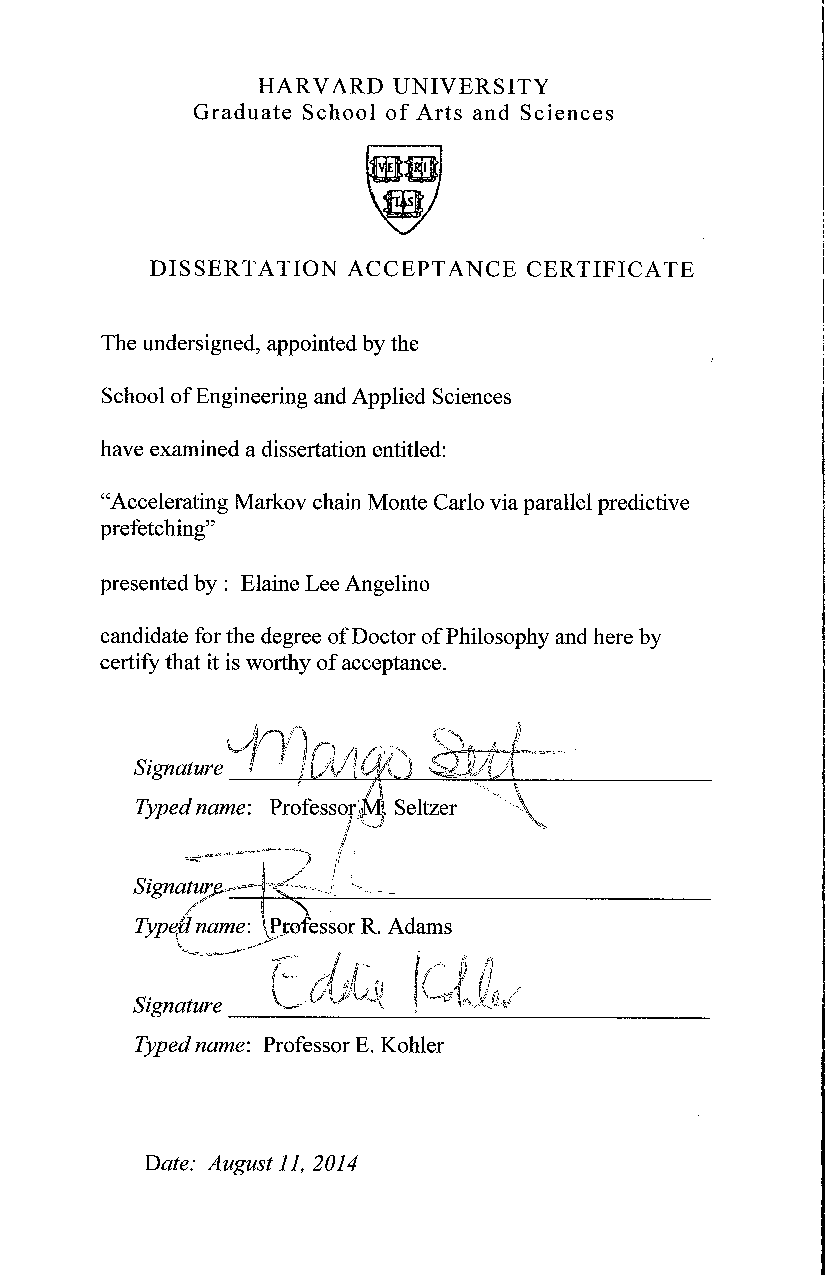
\includegraphics[]{figs/DAC-201408130921.pdf}
\end{center}
\end{figure}

\newpage
\thispagestyle{empty}
\pagestyle{empty}
\begin{center}
\end{center}

% page i:  title page (no page number)
\newpage
\setcounter{page}{1}
\begin{spacing}{2}

\begin{center}
\end{center}

\begin{center}
\end{center}


\begin{center}
Accelerating Markov chain Monte Carlo via parallel predictive prefetching \\
\end{center}


\begin{center}
A dissertation presented

by

Elaine Lee Angelino

to

The School of Engineering and Applied Sciences \\
\end{center}


\begin{center}
in partial fulfillment of the requirements

for the degree of

Doctor of Philosophy

in the subject of

Computer Science \\
\end{center}


\begin{center}
Harvard University

Cambridge, Massachusetts \\
\end{center}


\begin{center}
August 2014
\end{center}

\end{spacing}

\thispagestyle{empty}
\pagestyle{empty}


% page ii:  copyright notice (no page number)
\newpage

\null
\vfill

\copyright 2014 Elaine Lee Angelino

All rights reserved.

\thispagestyle{empty}
\pagestyle{empty}


% page iii:  abstract
\newpage

% max 350 words
\begin{spacing}{2}
\noi Dissertation Advisors \hfill  Author \\
\noi Professor Margo Seltzer and Professor Ryan P. Adams \hfill Elaine Lee Angelino

\begin{center}
Accelerating Markov chain Monte Carlo via parallel predictive prefetching \\
\end{center}

\begin{center}
Abstract \\
\end{center}

\begin{flushleft}
\hspace{15pt} We present a general framework for accelerating a large class of
widely used Markov chain Monte Carlo (MCMC) algorithms.
This dissertation demonstrates that MCMC inference can be accelerated 
in a model of parallel computation that uses speculation to predict and complete
computational work ahead of when it is known to be useful.
By exploiting fast, iterative approximations to the target density, we can
speculatively evaluate many potential future steps of the chain in parallel.
In Bayesian inference problems, this approach can accelerate sampling from the
target distribution, without compromising exactness, by exploiting subsets of data.
It takes advantage of whatever parallel resources are available, but produces
results exactly equivalent to standard serial execution.
In the initial burn-in phase of chain evaluation, it achieves speedup over
serial evaluation that is close to linear in the number of available cores.
\end{flushleft}

\end{spacing}
